\documentclass[a4paper]{article}
\usepackage[a4paper,margin=25mm]{geometry}
\usepackage{graphicx,subcaption}
\usepackage{amsmath,amsfonts}
\usepackage{qtree}
\usepackage{tikz}
\usetikzlibrary{arrows,arrows.meta,quotes}
\usepackage{varwidth}

\begin{document}

%%%%%%%%%%%%%%%%%%%%%%%%%%%%%%%%%%%%%%%%%%%%%
% Simple chunking grammar
\begin{figure}[hbt]
\centering
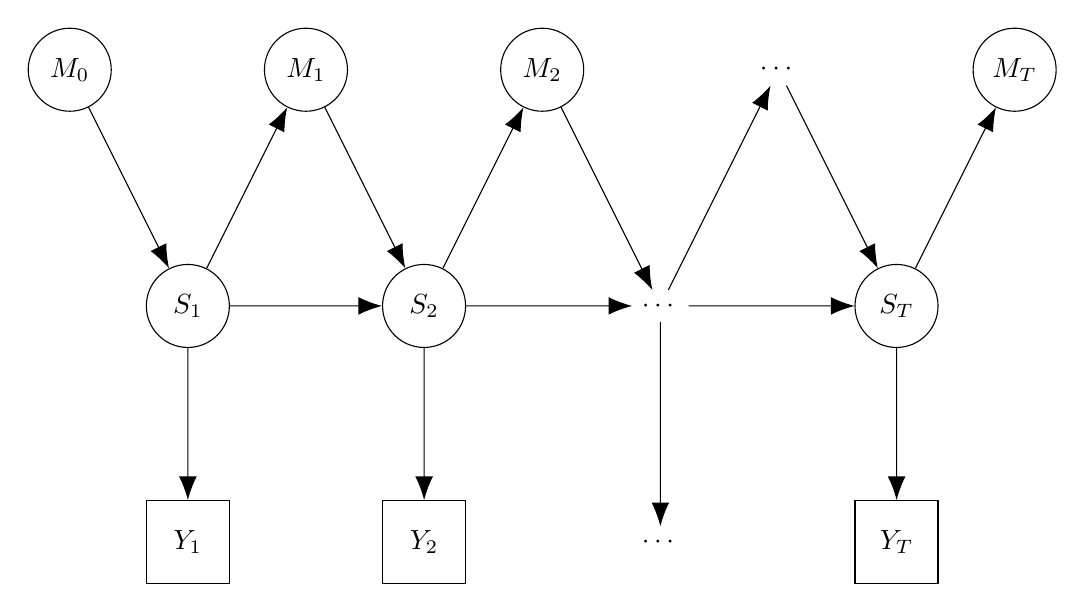
\begin{tikzpicture}[
  scale=1.5,
  cnode/.style={draw,circle,minimum size=3em,inner sep=3pt},
  snode/.style={draw,rectangle,minimum size=3em,inner sep=3pt}
]
  % tokens
  \node[snode] (y1) at (1,0) {$Y_1$};
  \node[snode] (y2) at (3,0) {$Y_2$};
  \node (ydot) at (5,0) {$\cdots$};
  \node[snode] (yT) at (7,0) {$Y_T$};

  % contexts
  \node[cnode] (m0) at (0,4) {$M_0$};
  \node[cnode] (m1) at (2,4) {$M_1$};
  \node[cnode] (m2) at (4,4) {$M_2$};
  \node (mdot) at (6,4) {$\cdots$};
  \node[cnode] (mT) at (8,4) {$M_T$};

  % states
  \node[cnode] (s1) at (1, 2) {$S_1$};
  \node[cnode] (s2) at (3, 2) {$S_2$};
  \node (sdot) at (5, 2) {$\cdots$};
  \node[cnode] (sT) at (7, 2) {$S_T$};

  % edges
  \draw[-{Latex[length=3mm]}] (m0) edge (s1);
  \draw[-{Latex[length=3mm]}] (s1) edge (y1);
  \draw[-{Latex[length=3mm]}] (s1) edge (m1);
  \draw[-{Latex[length=3mm]}] (s1) edge (s2);
  \draw[-{Latex[length=3mm]}] (m1) edge (s2);
  \draw[-{Latex[length=3mm]}] (s2) edge (y2);
  \draw[-{Latex[length=3mm]}] (s2) edge (m2);
  \draw[-{Latex[length=3mm]}] (s2) edge (sdot);
  \draw[-{Latex[length=3mm]}] (m2) edge (sdot);
  \draw[-{Latex[length=3mm]}] (sdot) edge (mdot);
  \draw[-{Latex[length=3mm]}] (sdot) edge (ydot);
  \draw[-{Latex[length=3mm]}] (mdot) edge (sT);
  \draw[-{Latex[length=3mm]}] (sdot) edge (sT);
  \draw[-{Latex[length=3mm]}] (sT) edge (yT);
  \draw[-{Latex[length=3mm]}] (sT) edge (mT);
\end{tikzpicture}
\end{figure}

\end{document}
